%%% This is an example file for the Auburn University style options
%%%       aums.sty (Masters Thesis)
%%%       auphd.sty (Ph.D. Dissertation)
%%%       auhonors.sty (Honors Scholar)

%%%To use it, please edit the necessary options, title, author, date, year, keywords, advisor, professor, etc. 

\documentclass[12pt]{report}
\usepackage{aums}       % For Master's papers
\usepackage{ulem}       % underlining on style-page; see \normalem below
\usepackage{url}
\usepackage{tikz}
\usepackage{pgf}
\usepackage{tocloft}     % Use tocloft to introduce single spacing on long chapter name
\setlength\cftparskip{-2pt}
\usepackage[nottoc,notlof,notlot]{tocbibind} 
\usepackage{graphicx}
\usepackage{subcaption}
\usepackage{amsmath}
\renewcommand\cftchapafterpnum{\vskip\baselineskip}  
\renewcommand\cftsecafterpnum{\vskip\baselineskip \normalfont}
\renewcommand\cftsubsecafterpnum{\vskip\baselineskip \normalfont}
\renewcommand\cftsubsubsecafterpnum{\vskip\baselineskip \normalsize}
\renewcommand\cftfigafterpnum{\vskip\baselineskip}
\renewcommand\cfttabafterpnum{\vskip\baselineskip}
\renewcommand{\cftpartleader}{\cftdotfill{\cftdotsep}} % for parts
\renewcommand{\cftchapleader}{\cftdotfill{\cftdotsep}} % for chapters
\usepackage{times}
\usepackage[a4paper,left=1in,right=1in,top=1.15in,bottom=1in]{geometry}
\usepackage{etoolbox}% http://ctan.org/pkg/etoolbox
\usepackage{titlesec}
\titleformat{\chapter}[display] %[display] puts the title chapter on a separate line
  {\singlespace\center}{\chaptertitlename\ \thechapter}{12pt}{\center} % Defines the Chapter title style and size
\titleformat*{\section} {\normalfont\fontsize{12}{12}}  % Added this line to describe section title,numbering and font styles
\titleformat*{\subsection} {\normalfont\fontsize{12}{12}}% Added this line to describe subsection title,numbering and font styles
\titleformat*{\subsubsection} {\normalfont\fontsize{12}{12}}% Added this line to describe subbsection title,numbering and font styles

%%%%%Format rules: Normal margins are 1 in. If you need to print with 1.5in margins, uncomment the line below
%\oddsidemargin0.5in \textwidth6in

%% If you do not need a List of Abbreviations, then comment out the lines below and the \printnomenclature line.
%%for List of Abbreviations information:  (see http://www.mackichan.com/TECHTALK/509.htm  )
\usepackage[intoc]{nomencl}
\renewcommand{\nomname}{List of Abbreviations}   	       
\makenomenclature 
%% don't forget to run:   makeindex ausample.nlo -s nomencl.ist -o ausample.nls
%% Also, if 




% May want theorems numbered by chapter
\newtheorem{theorem}{  \normalfont Theorem} [chapter]

% Put the title, author, and date in. 
\title{Test: A Software Signal Simulation of Low Earth Orbit Satellites for Investigative Analysis}
\author{Samuel McDougal} 
\date{Sometime Spring 2023} %date of graduation
\copyrightyear{2023} %copyright year

\keywords{LEO Satellites, USRP, Navigation, Signals of Opportunity}

% Put the Thesis Adviser here. 
\adviser{Scott Martin}


% Put the committee here (including the adviser), one \professor for each. 
% The advisor must be first, and the dean of the graduate school must be last.
\professor{Scott Martin}

\professor{David Bevly}

\professor{Brendon Allen}

\begin{document}

\begin{romanpages}      % roman-numbered pages 

\TitlePage 

\begin{abstract} 
Place the text of the abstract here. Headings come automatically.
\end{abstract}

\begin{acknowledgments}
acknowledgments
\end{acknowledgments}

\begin{singlespace}

\begin{center} 
\renewcommand{\cftchapfont}{}
\renewcommand{\cftchappagefont}{}
\renewcommand{\cfttoctitlefont}{\normalsize}% Remove \bfseries from ToC title
\renewcommand{\cftsecfont }{\normalsize}% Remove \bfseries from section titles in ToC
\renewcommand{\cftsecpagefont}{\normalsize}% Remove \bfseries from section titles' page in ToC
\tableofcontents 
\newpage
\renewcommand{\cftchapfont}{}
\renewcommand{\cftchappagefont}{}
\renewcommand{\cftloftitlefont}{\normalsize}% Remove \bfseries from lof title
\renewcommand{\cftsecfont}{\normalsize}% Remove \bfseries from section titles in lof
\renewcommand{\cftsecpagefont}{\normalsize}% Remove \bfseries from section titles' page in lof
\listoffigures
\newpage
\renewcommand{\cftchapfont}{}
\renewcommand{\cftchappagefont}{}
\renewcommand{\cftlottitlefont}{\normalsize}% Remove \bfseries from lot title
\renewcommand{\cftsecfont}{\normalsize}% Remove \bfseries from section titles in lof
\renewcommand{\cftsecpagefont}{\normalsize}% Remove \bfseries from section titles' page in lof
\listoftables
\end{center}
\end{singlespace}

\printnomenclature[0.5in] %used for the List of Abbreviations
\end{romanpages}        % All done with roman-numbered pages


\normalem       % Make italics the default for \em

 \chapter { Introduction}  % Use \\ for long titles  

\section { \normalfont Motivation}

Low Earth orbit (LEO) satellites for navigation have gained interest as an alternitive source of position, navigation and timing (PNT) to GNSS due to GNSS being susceptible to interferences such as jamming, spoofing, and multipath. Many current LEO satellites are not designed for navigation, however their signals have been exploited for opportunistic navigation. Many of these constellations have data messages that are unknown to the user which makes receiver design difficult. While there are a few high fidelity LEO simulators on the market, they can be expensive. These tools allow for testing of signal types before satellites are launched and signals can be replicated with prior knowledge of the signal. The development of a signal simulation tool that allows for testing of different signal types, satellite constellations, and receiver patterns is a necessaary tool for developing software and hardware receivers for LEO satellites.  

\section { Prior Work }

There are recent studies in positioning techniques with the growing interest in finding navigation possibilities with LEO satellites. Currently, global navigation satellite systems (GNSSs) are an integral part of modern society. Whether it is directions to the grocery store, land surveying, or autonomous vehicles, the knowledge of where something is and where it is supposed to go is important. Current GNSSs, such as Global Positioning System (GPS), use radio frequencies (RF) to determine position and velocity solutions. Methods for calculating positions and velocities from GPS satellites can be found in \cite{misraGlobalPositioningSystem2012}. 

The flexibility of a simulation tool is crucial. It saves time, money, and resources when testing different scenarios. One of the biggest advantages to this simulation tool is the ability to interchange different pieces quickly and efficiently. Whether it is the constellation type, data message, or signal structure, changes can be made easily to accommodate varying test plans. Current navigation simulation tools are mainly focused on GNSSs such as \cite{dongIFGPSSignal2003} and \cite{corbellDesignValidationAccurate2000}. One source, \cite{powellMultipleAntennaSoftwareGPS} designs a signal simulation tool for ``Rapid Testing of Interference Mitigation Techniques" for GPS. In his thesis, Powell outlines structures for creating a low cost signal simulation tool that can be used to test different scenarios. He begins by generating a file of simulation settings. This is followed by a scenario simulation where satellites are propagated, measurements are generated, and the navigation message populated. Next the signal is generated for the satellites in view and the data is stored in a bin file. GNSS signal simulators can also be used to test software defined receivers (SDRs). Powell validates his simulation by comparing the generated signal performance to the performance of a hardware gps receiver and examining the position, velocity, carrier to noise ratio, and Doppler frequencies. Powell found that the simulator described in his thesis was capable of producing realistic single and multi antenna signals. 


One of the main areas of research for LEO satellites is using the Doppler frequency measurements from the LEO satellites in order to gain a navigation solution \cite{hsuAssessmentUsingDoppler2014} \cite{psiakiNavigationUsingCarrier2021}. Doppler positioning has been used in GNSS \cite{bahramiGNSSDopplerPositioning}, and was even the precursor to GPS \cite{TransitSatelliteSpacebased}. The Transit satellite system was initially used for US naval ships to gain a rough position. In \cite{thompsonSingleDifferencedDoppler2021}, Thompson uses a double differenced Doppler technique to position a moving rover with LEO satellites using angle of arrival (AOA) estimates to remove the need of satellite state knowledge. The Argos satellite system uses Doppler measurements for animal tracking \cite{lopezImprovingArgosDoppler2014}
  

Another area of research with LEO satellites is to use their measurements and colaberate with IMUs for opportunistic navigation\cite{khalifeReceiverDesignDoppler2019} and \cite{tanNewMethodPositioning2019}. In \cite{moralesInertialNavigationSystem2018}, the Orbcomm constellation is used to to aid an inertial navigation system (INS) in a tightly-coupled fashion. Here they used the LEO satellite Doppler measurements and TLE files to estimate the position of a moving UAV without GNSS signals. For the experiment, the UAV was without GPS and had 2 Orbcomm satellites. They claim that this navigation framework lowered the UAV final position error by 72 percent when compared to solely using the IMU.

One possibility is to deploy a new constellation in LEO specifically for navigation  \cite{reidSatelliteNavigationAge2020}.


A LEO satellite signal simulator can be useful for testing different signal types, constellation geometries, and possible errors. The results of a simulation are only as good as the simulator itself. While high end signal simulators exist, they can be expensive and require technical prowess to operate. A low cost version can be valuable and still operate at a high level of fidelity with more ease of use. 

\section { Contributions}
This thesis will describe the process of designing a modular simulation tool for LEO satellites. The versitility of the simulator allows the user to test different scenarios. 
The contributions from this thesis are listed below:
\begin{itemize}
    \item Description of LEO satellite signal simulation tool that generates realistic IQ signals to be used for currrent and emerging constellations
    \item Investigation of USRP playback and record to realistic introduce hardware errors
    \item Examine possible positioning techniques for TDMA signals
    
\end{itemize}

\section{Thesis Outline}
In Chapter 2, the background of satellite orbits, signal types, and modulation types are discussed. In Chapter 3, the simulation tool is described in detail. Chapter 4 dives into the simulation and testing configurations used for this thesis. The results from the testing configurations are discussed in Chapter 5. Conclusions and future work are discussed in Chapter 6 followed by a list of references and an Appendix.


\chapter{Background}

\section{Satellite Based Navigation}\label{sec:satellitenav}
Satellite navigation employs trilateration as a way to solve the age old problem of determining where ones self is on planet Earth. Trilateration is the process of using ranges to determine unknown locations of things. In a 2-dimentional example, three transmitters produce circles with radius $r$. With knowledge of the location of the transmitters, the ranges can be used to calculate a circle around the transmitter. The intersection point of all three circles will enclose the positioning result. This can be seen in figure \ref{fig:Trilateration}.

\begin{figure}[h]
    \centering
    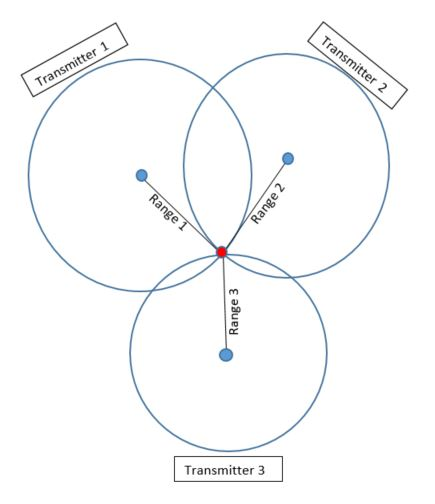
\includegraphics[width=4.0in]{Trilateration.JPG}
    \caption{Visual Depiction of Trilateration}
    \label{fig:Trilateration}
\end{figure}

The process of trilateration with satellites is the same except in 3-dimensional space. In the case of GPS, the satellites are the transmitters. Satellites make excelent transmitters in this case becasue of their ability to cover large areas continuously. An important point to mention is that the in the previous example it is assumed that the satellite and receiver are tied to the same clock. This means that the user has a perfect known time of the transmission of the signal from the satellite and perfect knowledge of the time of reception. However, this is not the case in real world examples. In fact, each satellite is tied to its own clock while each receiver is also tied to a separate clock. This offset in time can cause very large errors in positioning. To account for this, GPS ground stations survey and monitor the status of the satellite clocks to ensure maximum clock accuracy. While this takes care of the satellite part of the clock issue, the receiver clock still contains error. This error can be estimated along with the receiver states with the addition of a fourth measurement. With four unknown variables (receiver position $x$, $y$, $z$, and clock bias $b$), four measurements must be available in order to estimate the unknowns. 

Satellites use radio frequencies (RF) to transmit information to users on the surface of the Earth. These RF signals have encoded data called navigation messages that users can receive and unpack with specialized RF receivers. The navigation message can contain information such as satellite positions and velocities, clock corrections, and orbital parameters. These parameters are used for obtaining the precise location of satellites to obtain ranges that is used for solving the positioning problem. 

\section{Satellite Orbit Zones}

With regard to space vehicles, there are three main orbital zones. These zones are low Earth orbit (LEO), medium Earth orbit (MEO), and geosynchronous Earth orbit (GEO). These zones are differentiated by the altitude of the orbit above the surface of the Earth. Due to the nature of the orbits, the satellites in these orbital zones have varying mission types. Figure \ref{fig:satorbzone} gives a reference to each of the orbital zones. 

\begin{figure}
    \centering
    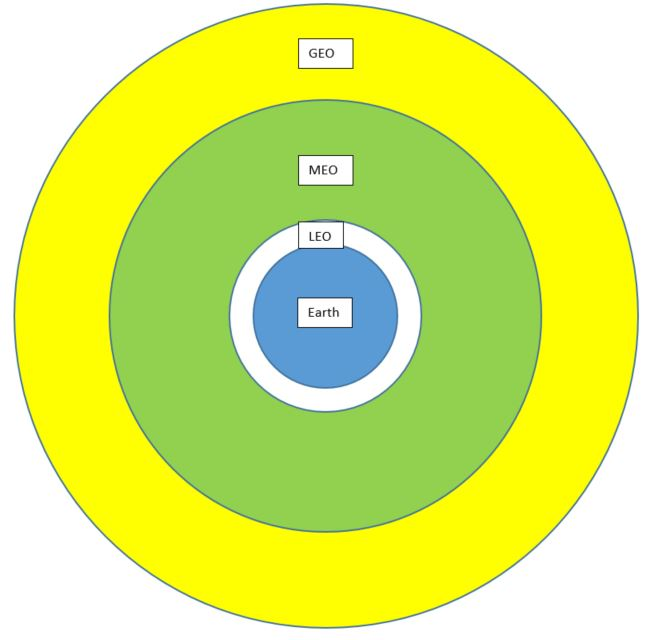
\includegraphics[width=4in]{satellite_orbit_zones.JPG}
    \caption{Visual Representation Orbit Zones}
    \label{fig:satorbzone}

\end{figure}


The furthest of the orbit zones is GEO. These satellites have an orbit altitude of 35,786 kilometers. Geosynchronous orbits are positioned at this precise altitude to allow the satellite orbit period to equal the same time as the rotation of the Earth for one day. The length of the orbit lasts one sidereal day. To an observer on Earth, the satellite would appear to stay in the same place throughout the course of its life. Another form of geosynchronous orbit is the geostationary orbit. Geostationary orbits are geosynchronous orbits specifically located at the Earth's equator and have a near zero inclination angle. GEO satellites are stationed where they are due to their specific mission type. One of the best attributes a GEO satellites has is a large footprint. The large footprint, along with the twenty four hour coverage, means these satellites are great for Earth observation. This also means that fewer satellites are required to be in orbit for full Earth coverage. Many of the current GEO satellites are used for weather, climate surveying, and oceanic observations \cite{usdepartmentofcommerceSatellites}. The Geostationary Operational Environmental Satellites (GOES) are the current Earth observation satellites operated by NASA and NOAA \cite{garnerGOESOverviewHistory2015}. GEO satellites are not conducive for navigation. This is due to the nature of the orbit. Since the orbit is so high, gaining a precise navigation message can be difficult due to loss of signal power and the amount of time it takes for the signal to reach Earth. Another issue with GEO satellites is the cost of launching these satellites. Launching satellites into GEO can cary a much higher price than satellites in LEO or MEO. These points were taken into consideration when GPS was first being thought about. (Maybe include an image of GEO coverage).

MEO is an orbital zone between LEO and GEO. MEO satellites have orbit altitudes between 2,000 kilometers and 35,000 kilometers. The orbit period for most MEO satellites is between 10 hours and 15 hours. Most of the satellites in MEO are navigation satellites. These constellations include GPS (USA), Galileo(European), GLONASS (Russia), and BieDou (China). Each country with GNSSs has designed them specifically for their own use. For example, GLONASS has an orbit altitude of 19,000 kilometers with satellites at specific inclination angles in order for the satellites to spend more time in view over Russia \cite{GLONASSInterfaceControl1998a}. GPS occupies MEO for many reasons, one being the number of satellites needed for global coverage. While more satellites are needed in MEO for global coverage than GEO, fewer are required than in LEO. GPS satellites have an orbit period just under 12 hours. With the orbit altitude and orbit period, 24 satellites are needed for global coverage in order to have at least 4 satellites in view to gain a positioning solution. However, with an orbit period of 12 hours, the observed Doppler frequencies of the satellites are low and can lead to poor velocity estimates. Next, LEO satellites are discussed.

\section{Low Earth Orbit Satellites}
LEO satellites are different than the previously mentioned zones. LEO satellites have orbits from 300 kilometers to 1500 kilometers. With this altitude, the orbit periods for LEO satellites tend to be 60 to 90 minutes, however the ammount of time that a satellite may be in view is lower. This poses issues in terms of global coverage. Satellite constellations with orbit periods on this time scale require far more satellites for full global coverage, and even more satellites for a possible navigation constellation. Reid et al says that it would take nearly 300 LEO satellites in order to provide global coverage \cite{reidSatelliteNavigationAge2020}. 
Current LEO constellations, such as Iridium and Orbcomm, are designed for communications. The Iridium constellation uses global coverage for satellite phones, where the Orbcomm constellation uses ``LEO satellites to provide worldwide geographic coverage for sending and receiving alphanumeric packages," \cite{orabiOpportunisticNavigationDoppler2021}. The data messages on these satellites are unknown as they are proprietary to the companies who sent them into space. This makes it difficult to design receivers and evaluate the navigation performance of these signals. However, a customized navigation message can be put on a similar signal. 

\subsection{Current LEO Constellations}
Current LEO constellations were not designed for navigation, specifically. Most are used for satellite communications, internet, and Earth observations. Some of the major constellations in LEO are Iridium/IridiumNEXT, Orbcomm, and Starlink. The IridiumNEXT \cite{IridiumNEXTReview2019}, which will be refered to as Iridium, is a telecomunications satellite network that comprises of 66 active satellites and 9 in-orbit spares. The 66 active satellites are grouped into 6 orbital planes with 11 satellites in each plane. These satellites are in near polar orbits which means the coverage at the poles is very high, however coverage at the equator is low. The main mission for Iridium is to provide telecomunications with sat-phones. Orbcomm is similar to Iridium as it is a satellite communications constellation, however the physical constellation is different. Orbcomm has 48 satellites with varying inclination angles. The Starlink constellation is a satellite broadband internet provider \cite{Starlink}. This constellation utilizes LEO orbit in an effort reduce latency with internet signals. Instead of using typical terestrial based techniques for internet providing, satellites are used to give coverage in places where internet may not be readily available. However to accomplish this goal, a massive constellation of satellites must be deployed. Currently, there are nearly 3,600 Starlink satellites in LEO with more planned for launch. All of these constellations have one thing in common. The original purpose of the mission was not for navigation. 

\section{Channel Access Methods}

Channel access methods are ways of communicating through mediums between multiple devices. Channel access methods allow users to send information back and forth between terminals. Channel access methods are used to manage telecomunications and wireless traffic. As there are multiple users trying to use or access the same information or services, channel access methods are used to differentiate between the users and the information being passed through the mediums. Three forms of channel access methods that will be examied are time division multiple access (TDMA), code division multiple access (CDMA), and frequency division multiple access (FDMA). 

\subsection{Time Division Multiple Access}\label{sec:TDMAsection}

Time division multiple access signals use time to differentiate incoming signals. This results in the signal being burst-like in nature and non-continuous between received signals. The carrier frequency, however, can remain the same accross all users. TDMA signals are typically used by telecomunication satellites such as Iridium. These signals are ideal for communications because as the users are separated in time, the possibility of data interference between users is low. A visual representation of a TDMA signal can be seen in figure \ref{fig:TDMAVisual}.
\begin{figure}[h!]
    \centering
    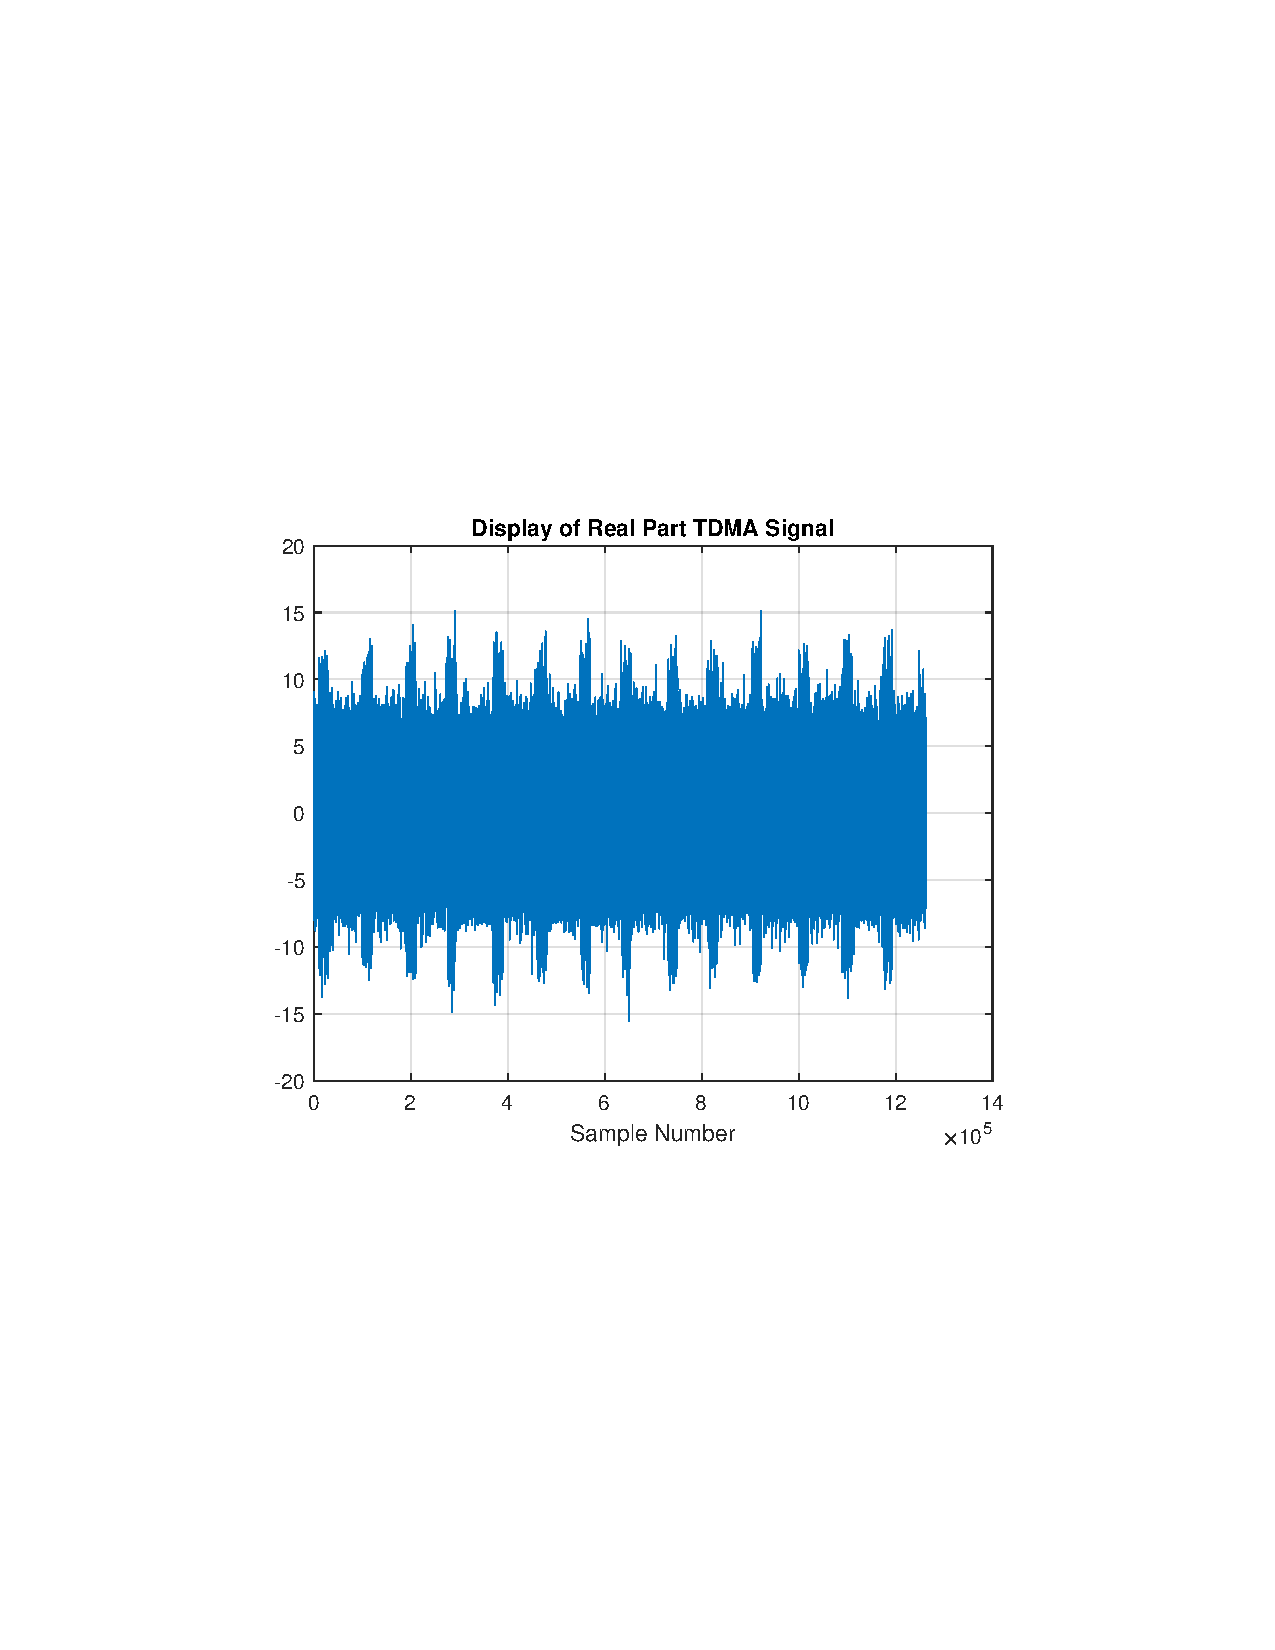
\includegraphics[width=5in]{TDMA_signal}
    \caption{Visual Representation of TDMA Signal}
    \label{fig:TDMAVisual}
\end{figure}
The burst nature of the signal can be seen in this image. The large bulk of the signal is noise, and the parts extending out of the noise are the the bursts. This shows the separation of the signal accross time. 

\subsection{Code Division Multiple Access}

Similar to TDMA, CDMA signals are broadcast at a single carrier frequency. However unlike TDMA, CDMA signals use deterministic binary sequence codes to differentiate signals. In the case of satellites, each satellite is given its own pseudo-random noise (PRN) sequence. These codes are designed specifically to have very low cross correlation in order to eliminate errors and deciphur different satellite's signals in the same frequency band. Cross correlation is a measure of similarity between two or more sequences. They also employ a high level of autocorrelation which is important for signal tracking \cite{goldOptimalBinarySequences1967}. Two notable GNSSs that employ CDMA signals are GPS and Galileo.

\subsection{Frequency Division Multiple Access}

Similar to CDMA, FDMA signals are continuous. However, these signals are not transmitted at the same carrier frequency. FDMA signals use different freqency bands to transmit data and information. For example, FM radio uses this technique to differentiate between radio channels such as sports talk radio and the local country music station. Similar to the radio in a car, some satellite constellations use the same idea, except each satellite transmits at a specific frrequency band. For example, GLONASS uses FDMA signals for their satellites but also use a PRN code. Unlike GPS, however, they all transmit the same PRN sequence \cite{GLONASSSignalPlan}. 

\section{Modulation}
In the world of satellite navigation and telecomunications, the term modulation refers to the process of incorporating data onto a carrier wave. This data is represented in binary form through 1's and 0's. When a signal is generated, these ones and zeros are converted into 1's and -1's for the purpose of signal modulation. Three forms of modulation include amplitude shift keying (ASK), frequency shift keying (FSK), and phase shift keying (PSK). ASK is the process of changing the amplitude of the sine wave to represent ones and zeros of binary data, FSK is the process of changing the frequency of the sine wave to represent ones and zeros of binary data, and PSK changes the phase of the signal to incorporate the data. ASK and FSK are shown in figure \ref{fig:ASKsig} and \ref{fig:FSKsig} respectively.

\begin{figure}[h]

    \centering
    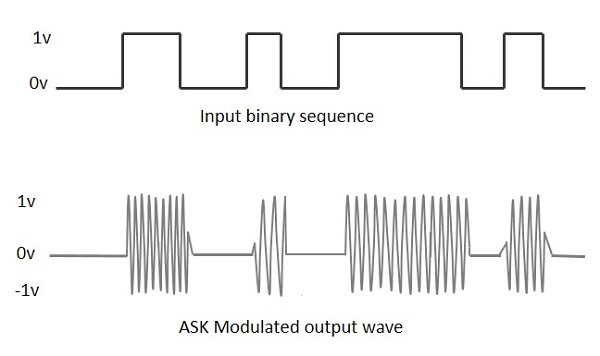
\includegraphics[width=4.0in]{ask_modulated_waveform.jpg}
    \caption{Amplitude Shift Keying Visualization \cite{AmplitudeShiftKeying} }
    \label{fig:ASKsig}

\end{figure}

\begin{figure}[h]

    \centering
    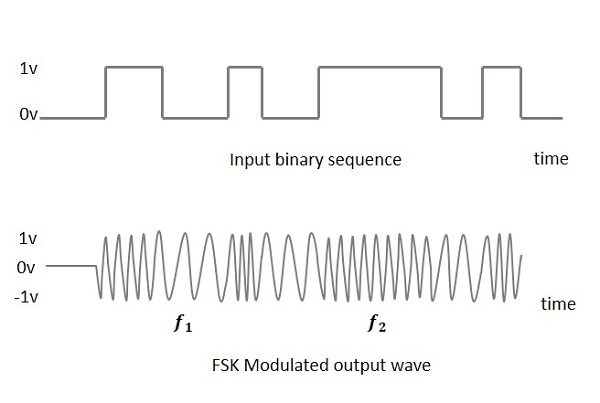
\includegraphics[width=4.0in]{fsk_modulated_output_wave.jpg}
    \caption{Frequency Shift Keying Visualization \cite{FrequencyShiftKeying} }
    \label{fig:FSKsig}

\end{figure}

Two forms of PSK are binary phase shift keying (BPSK) and quadrature phase shift keying (QPSK) and will be discussed below.

\subsection{Binary Phase Shift Keying}

BPSK is accomplished by shifting the phase of the signal by 180 degrees depending on the sign of the data bit. For example, when the sign of the data bit in the message changes, the phase of the signal flips by 180 degrees. By doing so, only one bit can be modulated per symbol. GPS uses BPSK modulation for its CA codes, navigation data, and P(Y) codes (encrypted message). BPSK is used due to its resiliance to bit error rate. A visual depiction of the BPSK signal can be seen in figure \ref{fig:BPSKsig}. In the figure, the phase change of the signal by 180 degrees can be seen at the change of each data bit. 

\begin{figure}[h]
    \centering
    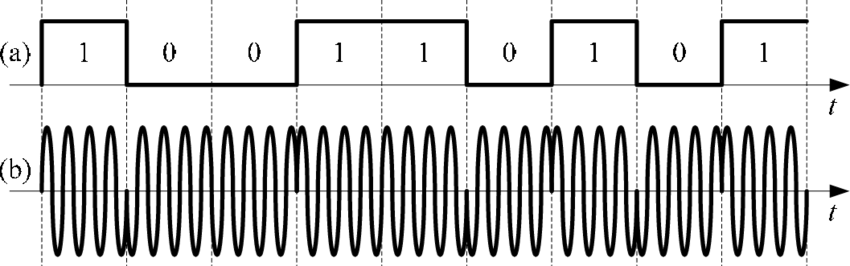
\includegraphics[width=4.0in]{Example-of-BPSK-modulation-format-a-binary-signal-and-b-BPSK-modulated-signal.png}
    \caption{Binary Phase Shift Keying Visualization \cite{mahdirajiAdvancedModulationFormats2010} }
    \label{fig:BPSKsig}
\end{figure}
\subsection{Quadrature Phase Shift Keying}
\label{sec:QPSK}

QPSK modulation uses 4 possible phases of the signal to to modulate the data onto the carrier wave. The phase possibilities are 90 degree offsets. With this, two bits are transmitted in one symbol. This allows for faster data rates of the signal. Figure \ref{fig:QPSKmod} shows a visual example of QPSK modulation.

\begin{figure}[h]
    \centering
    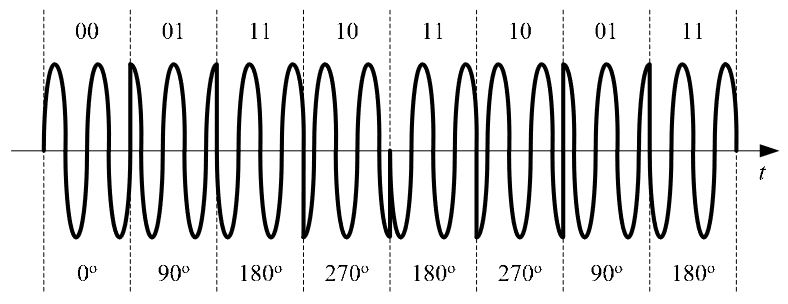
\includegraphics[width=4.0in]{QPSK_sig.JPG}
    \caption{Quadrature Phase Shift Keying Visualization \cite{mahdirajiAdvancedModulationFormats2010} }
    \label{fig:QPSKmod}
\end{figure}


\chapter {Simulation Tool}
In this section, the function and versitility of the simulator will be described.

\section{Simulator Overview}

The overall structure of the simulation is shown in figure \ref{fig:SimDiagram}.
\begin{figure}[ht]
    \centering
    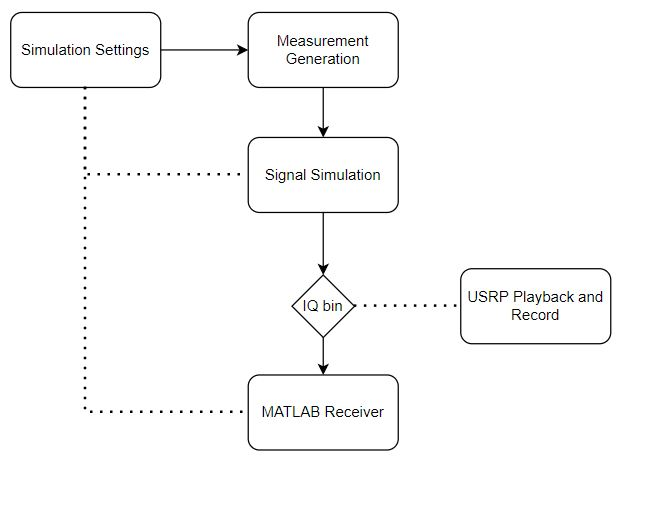
\includegraphics[width=4.0in]{OverallSimulationDiagram}
    \caption{Overall Simulation Diagram}
    \label{fig:SimDiagram}
\end{figure}

The simulation begins with the simulation settings file. This is a configuration file where all of the settings will be declared. This includes, but is not limited to, the satellite trajectories, signal power, and simulation length. The simulation settings file is fed into each block of the simulation tool. First, it goes into the measurement generation block. The measurement generation block is where the satellite positions and velocities are propagated, ranges and range rates are calculated, and transmit and received times are produced. Those terms are pushed into the signal simulation. Inside the signal simulation block the signal is generated and packaged into a bin file. Finally, the bin file is sent to a receiver where it is picked up, processed, and decoded to produce measurements. The following subsections will address each part of the simulation.

\section{Simulation Settings}

The simulation settings is a configuration file where all of the constants and settings used throughout the simulation are declared. All of the settings are stored in a MATLAB structure labeled `settings'. A MATLAB structure is a data storing type where different variables can be tied to one overall variable. The purpose for incorporating all of the settings and variables in one script is to ensure all variables are in one place. This helps the user find a variable quickly and efficiently. It also aids the user by ensuring consistency across all parts of the simulation. 

In part, the simulation settings allow this tool to be modular. The file begins with constants such as the speed of light, rotation rate of the Earth, Earth gravitational constants, and time constants. These will likely stay the same across any and all simulations. Next is the input of user time. This time is in the format of year, month, day, hour, minute, second and determines the start time of the simulation. Following the time starting point is the duration of the simulation in seconds and the measurement simulation sampling frequency in hertz. The next setting is the user position. Currently, the simulation allows for a static receiver with initial position defined in latitude, longitude, and altitude (LLA); however, the addition of a dynamic receiver can be made. Once the LLA position has been defined, the Earth centered Earth fixed (ECEF) position can be calculated. Next is the introduction of measurement error terms. The first set are weather terms for the error caused by the troposphere \cite{misraGlobalPositioningSystem2012}. These inputs are temperature in Celsius and Kelvin, barometric pressure in millibars, and humidity as a percentage. This is followed by clock settings. Here the user declares what type of clock to use and whether the clock error is to be simulated, indicated by an on or off switch. The clock is modeled based on \cite{}. Next is the satellite propagation settings. This simulation uses a simplified general perturbation (SGP) model for calculating satellite positions and velocities. Here the user will input a two line element (TLE) file name along with other information used in parsing the TLE. The propagation settings also includes a mask angle setting. The mask angle input is in degrees and allows the user to reject  satellites under the specified elevation angle. After the satellite propagation settings are the signal settings. Here the user decides the carrier frequency, sampling frequency, code frequency, number of symbols in the data message, and signal type. One specific signal type is time division multiple access (TDMA). A TDMA signal uses time slots in the form of bursts to decipher different signals, whereas frequency division multiple access (FDMA) uses different frequency channels. If the declared signal type is TDMA, then the burst period will need to be calculated. This is followed by the noise and signal power.

The simulation settings file is integral to this simulation tool. All other components of this simulator are dependent on it. These specific dependencies will be explained in detail in the remaining subsections.

\section{Measurement Simulation}
\subsection{Introduction}
The next block of the simulation tool is the measurement generation. The measurement generation is where satellites are propagated, ranges, range rates, and times are calculated. The purpose of this section is to have a set of truth values that will be used later in the simulation. The block diagram for the measurement generation is shown in figure \ref{fig:MeasBlock}.

\begin{figure}[h]
    \centering
    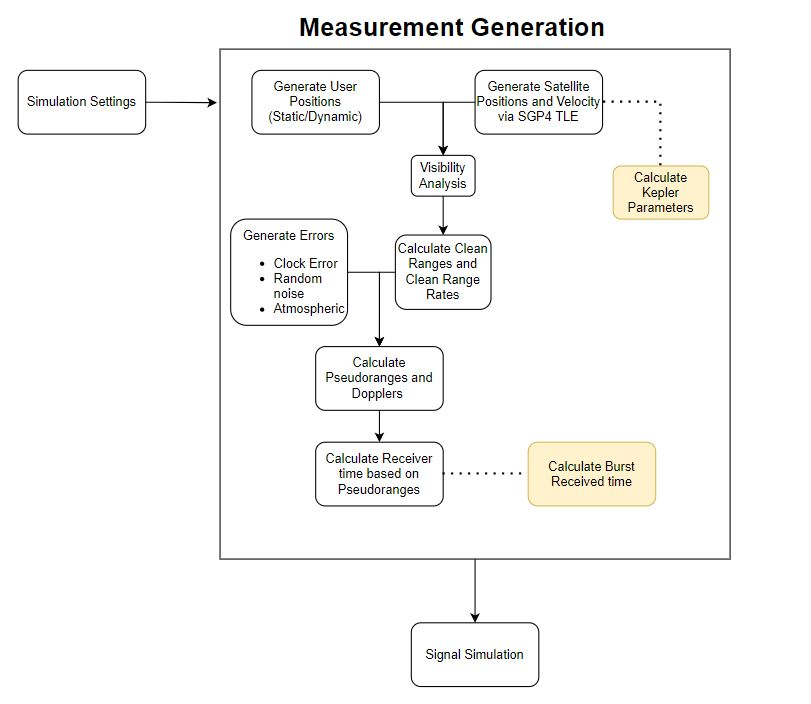
\includegraphics[width=5in]{MeasurementGenBlockDiagram}
    \caption{Measurement Generation Block Diagram}
    \label{fig:MeasBlock}
\end{figure}

The measurement simulation begins with the input of the simulation settings file. The following settings are the main terms used in the measurement simulation:
\begin{itemize}
    \item User Position and Velocity
    \item Year, Month, Day, Hour, Minute, Second of begining of simulation
    \item Simulation length in seconds
    \item Sampling frequency of measurement simulation
    \item Weather settings
    \begin{itemize}
        \item Temperature in Kelvin
        \item Temperature in Celcius
        \item Barometric pressure in millibars
        \item Humidity as a percentage
    \end{itemize}
    \item Clock settings
     \begin{itemize}
        \item Receiver clock type
        \item Satellite clock type
     \end{itemize}
     \item Satellite propagation settings
     \begin{itemize}
        \item TLE file name
        \item TLE Objects
        \item TLE exclude numbers
        \item Mask angle
        \item Augmented number of satellite orbital planes
        \item Augmented number of satellites per orbital plane
        \item Augmented inclination angle 
        \item Augmented orbit altitude in meters 
     \end{itemize}
     \item Burst time (seconds)
     \item Toggle switches
     \begin{itemize}
        \item Receiver type (static/dynamic)
        \item Receiver clock (on/off)
        \item Satellite clock (on/off)
        \item Tropospheric error (on/off)
        \item Satellite augmentation (on/off)
        \item Additional Noise (on/off)
     \end{itemize}
\end{itemize}

A breakdown of the following subsections are as follows: satellite propagation, error generation, measurement calculation, and final outputs from the measurement simulation. 

\subsection{Satellite Propagation}
For this simulation tool, the simplified general perturbation (SGP4) two line element (TLE) satellite propagator is used. SGP4 is a propagation technique used to calculate positions and velocities of satellites, space debris, and orbital junk. The SGP4 TLE propagator is used to calculate near Earth objects which are classified as having orbit periods less than 225 minutes. This corresponds well for LEO satellites as the orbital period is typically between 90 and 120 minutes. The perturbations accounted for in SGP4 include solar radiation, drag, and gravitational perturbations caused by the sun and the moon. SGP4 uses TLE files as a basis of propagation. TLE files are generated for tracking space objects. These files can be found on CelesTrak.org and can be pulled in the form of a text file for current day data. TLE files are 2 lines of 69 columns with orbital and satellite data. The information inside the TLE files is shown below.
\begin{center}
    \begin{tabular}{|c|c|c|}
        \hline
        Columns Used & Term & Line Number \\
        \hline
        1 & Line number & 1 \\
        \hline
        3-7 & USSC satellite catalog number & 1 \\
        \hline
        8 & Classification & 1 \\
        \hline
        10-11 & Launch year & 1\\
        \hline
        12-14 & Launch number of year & 1 \\
        \hline
        15-17 & Part of launch & 1 \\
        \hline 
        19-20 & Epoch year & 1 \\
        \hline
        21-32 & Epoch day plus fractional & 1 \\
        \hline
        34-43 & Balistic coefficient & 1 \\
        \hline
        45-52 & Second derivative of mean motion & 1 \\
        \hline
        54-61 & B-star drag term & 1 \\
        \hline
        65-68 & Element Set number & 1 \\
        \hline
        69 & Checksum & 1 \\
        \hline\hline
        1 & Line number & 2 \\
        \hline
        3-7 & USSC satellite catalog number & 2 \\
        \hline
        9-16 & Inclination angle & 2 \\
        \hline
        18-25 & RAAN & 2 \\
        \hline
        27-33 & Eccentricity & 2 \\
        \hline
        35-42 & Argument of perigee & 2 \\
        \hline
        44-51 & Mean anomaly & 2 \\
        \hline
        53-63 & Mean motion & 2 \\
        \hline
        64-68 & Revolution number at epoch & 2 \\
        \hline
        69 & Checksum & 2 \\
        \hline\hline
        
    \end{tabular}

\end{center}

The TLE files found on CelesTrak.org are for current space objects and satellite constellations. This simulation tool includes the option to augment the pre-existing satellite constellations with more satellites. In this case, TLEs are generated based on input values declared by the user. These terms are then used for the propagation of the satellites along with the following settings:
\begin{description}
    \item[TLE file name] This is the name of the text file with the list of TLEs for the satellite constellation being examined.
    \item[Objects] The objects are the names of the satellites in the constellation. This needs to be declared for when the TLE file is parsed.
    \item[Exclude] In some instances, there will be duplicates of satellites in a TLE file. These satellites need to be ignored when generating satellite data. Another instance would be when a collision has occured with a satellite and the data tracked in the TLE is the crash object and the debris caused by it.
    \item[Simulation length] This is the length of the simulation in seconds as previously mentioned.
    \item[Simulation start time] The begining time of the simulation in year, month, day, hour, minute, seconds at UTC time. Primarily the hour-minute-second because this is used for determining how far past the current epoch the satellite is being propagated at. 
    \item[Measurement sampling frequency] This is the rate at which measurements are generated for the simulation. 
    \item[Receiver Position] A vector of predetermined receiver positions in the ECEF coordinate frame. For a static receiver the vector of user positions has been generated forward for the length of the simulation at the desired sampling frequency. The vector of user positions will remain the same through the simulation as the points are not changing in the ECEF frame. For a dynamic receiver the user will input a pre-recorded or generated path that has been sampled to the sampling frequency of the simulation.
    \item[Mask angle] The mask angle is declared in degrees. A mask angle is a term used to describe the the range of view that a receiver will receive a signal from. For example, if a receiver was in an open area where the horizon is unobstructed, then the mask angle could be chosen to be zero degrees. However in most situations, the mask angle will be higher than zero due to unrealistic field of view of satellites at the horizon.
    \item[Augmentation settings] As previously mentioned, the simulation tool allows the user to declare additional satellites to the current constellation being examined. The inputs from the user are number of orbital planes, number of satellites per plane, inclination angle, and orbit altitude. This feature is important for examining future constellations or investigating the performance of constellations that have not been conceived.
\end{description}

The SGP4 TLE propagator begins with the input of the TLE file and the simulation settings. The TLE file is parsed and a MATLAB structure is used to store each element for each individual satellite. If declared the augmented satellite orbits are generated and added to the TLE structure. An Earth orientation parameters (EOP) file is hardcoded into the simulator, however this file needs to be updated periodically manually by the user. This data can also be aquired from the CelesTrak website. Time units are established and the begin time, end time, and time-step are calculated along with the time vector for the simulation. Memory is allocated for the position and velocity of each satellite in the ECEF and Earth centered inertial (ECI) coordinate frames. Next the satellites are propagated one at a time for the length of the simulation. The position and velocity vectors are put into the respective variable for ECEF and ECI. The azimuth and elevation angle are calculated for each satellite at each timestep of the simulation using the satellite positions and user positions. The elevation angles will have values $-90^{\circ} < El < 90^{\circ}$. A visibility analysis can be performed with the elevation angles. The visibility analysis takes the elevation angles and finds the satellites that are above the mask angle to eliminate them from the simulation. The output of the visibility analysis is a list of satellites and the times that they are in view. This greatly reduces the computation time for the rest of the simulation because the simulator does not calculate measurements or signals for the out of view satellites. New variables of satellite positions and velocities are generated and filled for satellites that are in view. Mathematically this is represented in equation \ref{eqn:VisAnal} where \textit{MA} is the mask angle and \textit{El} is the elevation angle.
\begin{equation}
    SV_{data} = 
    \left\{
        \begin{array}{lr}
            Fill cell, MA < El < 90^\circ \\
            NaN, MA > El
        \end{array}
    \right.
    \label{eqn:VisAnal}
\end{equation}
Each satellite state component ($x_{sv},y_{sv},z_{sv}$ and $\dot{x_{sv}},\dot{y_{sv}},\dot{z_{sv}}$) for both coordinate frames are saved into individual matricies. The dimensions for each matrix is $m \times n$, where \textit{m} is the length of the time vector and \textit{n} is the number of satellites propagated.
Figure \ref{fig:bothpropsats} shows the propagated satellite orbits in view above Auburn Alabama for the Iridium and Orbcomm constellations over the duration of a 15 minute simulation. 

\begin{figure}[ht]
    \centering
    \begin{subfigure}{.4\textwidth}
        \centering
        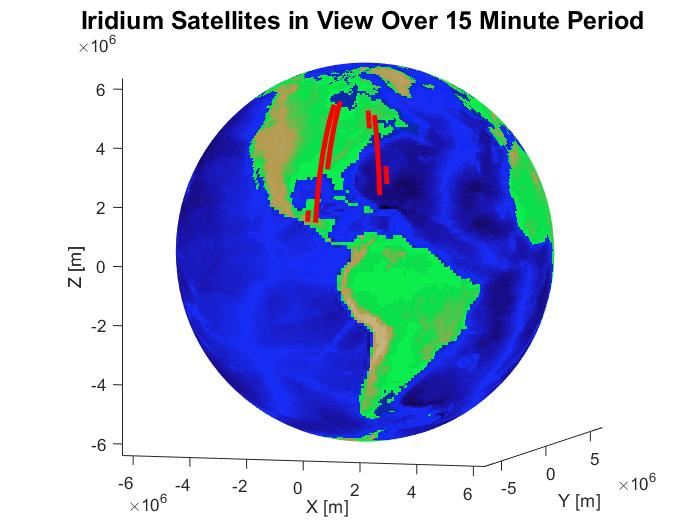
\includegraphics[width=\textwidth]{Iridium_sats_over_auburn.jpg}
        \caption{Propagated Iridium Satellites in View}
        \label{fig:IridSatsOverAub}
    \end{subfigure} %
    \begin{subfigure}{.42\textwidth}
        \centering
        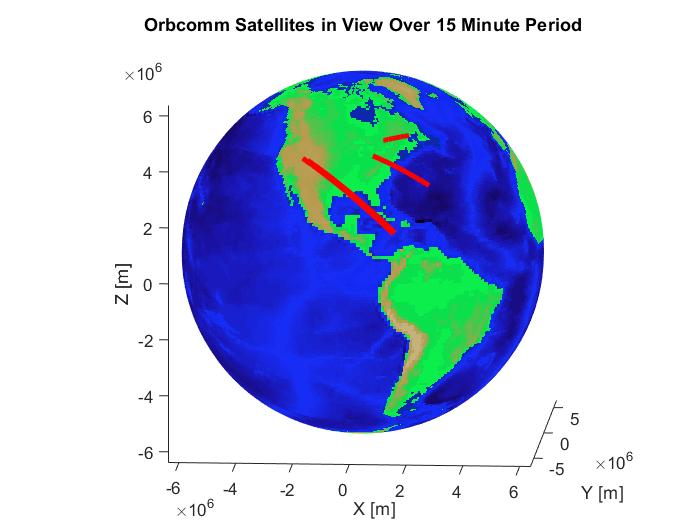
\includegraphics[width=\textwidth]{Orbcomm_sats_over_auburn.jpg}
        \caption{Propagated Orbcomm Satellites in View}
        \label{fig:OrbSatOverAub}
    \end{subfigure}
    \caption{Propagated Satellites from SGP4}
    \label{fig:bothpropsats}
\end{figure}

The final outputs from the satellite propagation stage are as follows:
\begin{description}
    \item[Satellite Positions] The 3-dimensional satellite position vectors in ECEF and ECI for all satellites propagated.
    \item[Satellite Velocity] The 3-dimensional satellite velocity vectors in ECEF and ECI for all satellites propagated.
    \item[Elevation Angle] The elevation angle of the satellites with respect to the user position.
    \item[In-view states] The 3-dimensional satellite position and velocity vectors in ECEF and ECI for in-view satellites.
\end{description}

With the satellites propagated and a visibility analysis conducted, the next step is to calculate errors.

\subsection{Error Generation}

After the visibility analysis, errors will be generated for the satellites that are in view. Measurement errors need to be calculated for computing the received time of the signal. Two primary sources of error modeled in this thesis are clock error and tropospheric delay. As previously discussed, clocks are imperfect and have a tendency to have a bias and drift over time due to the oscillator inside of the clock. For example, satellite clocks are more accurate because they use atomic clocks where receivers typically use a crystal oscillator. The tradeoff is cost because atomic clocks are significantly more expensive than crystal oscillators. The satellite clock and receiver clock will have independed biases and drifts. The satellite is assumed to be capable of knowing and transmitting its bias and drift, while the receiver clock must be estimated by the receiver. Tropospheric delay is the error caused by gasses in the Earth's atmosphere. The atmosphere is composed of dry gasses and water vapor. These molecules have a refractive properties that effect RF signals. The input settings for these errors are as follows:

\begin{description}
    \item[Clock Toggle] There is a setting in the simulator where the user can choose to turn on or off the generated clock error. There is a switch for both the satellite clocks and the receiver clocks.
    \item[Clock Type] The user will declare what type of clock to model for both the satellite and the receiver. Inside the clock error generation function, there are pre-set clocks and clock terms.
    \item[Troposphere Toggle] There is a toggle switch to turn the tropospheric delay on or off.
    \item[Temperature] There are two inputs for temperature. One is in Kelvin and the other is in degrees Celcius. 
    \item[Atmospheric Pressure] The atmospheric pressure is delcared in millibars.
    \item[Humidity] The humidity of the current time of simulation is input as a percentage.     
\end{description}


The first error generated is clock error. The clock bias and clock drift are calculated for each satellite in view over the simulation based on the clock type described by the user. Next the receiver clock is modeled and the bias and drift are generated. As previously mentioned, this option can be turned off and the errors will be incorporated as zeros in the simulation. The current clock types in the simulator are shown in the table \ref{table:ClockTypes}. 

\begin{center}
\begin{tabular}{|c|c|}
    \hline
    Oscillator & Acronym\\
    \hline\hline
    Cesium & Cesium\\
    \hline
    Rubidium & Rubidium\\
    \hline
    Oven Controlled Crystal Oscillator & OCXO\\
    \hline
    Temperature Controlled Crystal Oscillator & TCXO\\
    \hline
\end{tabular}
\label{table:ClockTypes}

\end{center}

Next the tropospheric delay is calculated from the settings defined previously. The model used is found in \cite{misraGlobalPositioningSystem2012}. In this thesis the tropospheric delay is modeled as a function of elevation angle with the definition of obliquity factors. This is also refered to as mapping functions. The equation for tropospheric delay is 

\begin{equation}
    \tilde{T} = \tilde{T}_{z,d} \cdot m_d(el) + \tilde{T}_{z,w} \cdot m_w(el)
    \label{eqn:TropError}
\end{equation}
where $\tilde{T}_{z,d}$ and $\tilde{T}_{z,w}$ are the dry and wet tropospheric zenith delay, respectively, and $m_d$ and $m_w$ are the mapping functions for the dry and wet components. The Saastamoinen model is used for calculating the dry tropospheric zenith delay is calculated as

\begin{equation}
    \tilde{T}_{z,d} = 0.002277(1+0.0026cos2\phi +0.00028H)P_0
    \label{eqn:DryZenith}
\end{equation}
where $\phi$ is the latitude of the receiver, \textit{H} is the height of the receiver, and $P_0$ is the total pressure. 
The wet tropospheric zenith delay is calculated as 

\begin{equation}
    \tilde{T}_{z,w} = 0.002277 \left( \frac{1255}{T_0} + 0.05 \right) e_0
    \label{eqn:WetZenith}
\end{equation}
where $T_0$ is the temperature in Kelvin and $e_0$ is the partial pressure due to water vapor.

The mapping function for the dry delay is 
\begin{equation}
    m_d(el) = \frac{1}{sin(el)+\frac{0.00143}{tan(el)+0.0445}}
    \label{eqn:drymapping}
\end{equation}
and the mapping for the wet delay is
\begin{equation}
    m_w(el) = \frac{1}{sin(el)+\frac{0.00035}{tan(el)+0.017}}
    \label{eqn:wetmapping}
\end{equation}

Finally, the addition of white Gaussian noise is added for errors not modeled (i.e. Ionosphere delay, multipath, etc).

The final outputs of the error generation are as follows
\begin{description}
    \item[Satellite Clock Error] The error caused by satellite clocks. This is a MATLAB structure that is indexed for each satellite in view with fields of bias and drift. The error caused by bias and drift have units of meters and meters per second, respectively.
    \item[Receiver Clock Error] The error caused by the receiver clock. The receiver clock error is saved into the same structure as the satellite clock error labeled 'ClockError'. The units for error caused by the bias and drift are also meters and meters per second, respectively.
    \item[Tropospheric Error] The error caused by the troposphere. This will be a matrix of tropospheric error for each satellite in view at each time step of the simulation. The units for tropospheric error are output in meters.
\end{description}

\subsection{Measurement Calculations}
With the errors generated, the measurements are calculated. The measurement calculations section only has one input from the simulation settings. This input is the burst timing of the signal. The user will declare this in terms of seconds. This step needs to be included because the receive time of the signal is calculated based on the satellite burst time. This will be discussed later in the section. This subsection will give the equations used for calculating true ranges and range rates, pseudoranges and pseudorange rates, Doppler frequency, received time, and Kepler orbital parameters. 

The true satellite to receiver ranges are calculated along with the range rates. Their equations are show below.
\begin{equation}
    r = \sqrt{(x^{(k)}_{sv} - x_u)^2 + (y^{(k)}_{sv} - y_u)^2 + (z^{(k)}_{sv} - z_u)^2}
    \label{eqn:rangeeqn}
\end{equation}
\begin{equation}
    \dot{r} = (\mathbf{v}^{k} - \mathbf{v}_r) \cdot \mathbf{1}
    \label{eqn:rangerate}
\end{equation}

Having generated ranges, range rates, and errors, the receiver observed pseudorange and Doppler measurements can be calculated. The equations for pseudorange, pseudorange rate, and Doppler are equations \ref{eqn:pseudorange}, \ref{eqn:pseudorangerate}, and \ref{eqn:doppler}, respectively.
\begin{equation}
    \rho^{(k)} = r^{(k)} - b_{sv} + b_r + T +\epsilon
    \label{eqn:pseudorange}
\end{equation}

\begin{equation}
    \dot{\rho} = \dot{r} + \dot{b_r} - \dot{b_{sv}} + \epsilon
    \label{eqn:pseudorangerate}
\end{equation}

\begin{equation}
    f^{(k)}_{Doppler} = \frac{\dot{\rho}}{-\lambda}
    \label{eqn:doppler}
\end{equation}


Where in equation \ref{eqn:pseudorange}, $\rho$ is the observed pseudorange calculated from range \textit{r} to the $k^{th}$ satellite, satellite clock bias $b_{sv}$, receiver clock bias $b_{r}$ in meters, troposphere delay \textit{T},  and additional noise for errors not modeled $\epsilon$. In Equation \ref{eqn:pseudorangerate}, $\dot{r}$ is the calculated range rate, $\dot{b_r}$ is the receiver clock drift, $\dot{b_{sv}}$ is the satellite clock drift, and un-modeled errors $\epsilon$, all with units of meters per second. In equation \ref{eqn:doppler}, $f^{k}_{Doppler}$ is the Doppler frequency of the $k^{th}$ satellite, $\dot{\rho}$ is the pseudorange rate, and $\lambda$ is the wavelength of the carrier. Once the pseudorange and Doppler measurements have been calculated, the observed receive time of the signal can be calculated. It is important to calculate the received time of the signal based on the pseudorange because the signal is generated at the received level. The received time is calculated as 
\begin{equation}
    t_{rx} = t_{tx} + \frac{\rho}{c}
    \label{receivetime}
\end{equation}
where $t_{tx}$ is the transmit time, $\rho$ is the pseudorange calculated in equation \ref{eqn:pseudorange}, and \textit{c} is the speed of light. For a TDMA signal, burst timing needs to be calculated. For example, if the burst timing 70 milliseconds, then a burst will at $t=0s$, $t=0.07s$, $t=0.14s$ and so on. For this instance, the received time of the signal is also calculated on the burst interval using equation \ref{receivetime}.

An option the user has for a data message type is Kepler orbital parameters or classical orbital elements (COE). The calculation of COE uses the ECI satellite positions and velocities calculated previously. These terms are: \textit{h} magnitude of angular momentum; \textit{e} eccentricity; \textit{RAAN} right ascension of the ascending node, \textit{i} inclination angle; \textit{w} argument of perigee; \textit{TA} true anomaly; \textit{a} semi major axis. This process is described in. \cite{curtisOrbitalMechanicsEngineering2008}.

The final outputs from the measurement generation are as follows:
\begin{description}
    \item[Satellite States] The positions and velocities of satellites that are in view for the duration of the simulation in meters and meters per second, respectively for both the ECEF and ECI frames. 
    \item[True Range] The true range of the satellite to the receiver in meters.
    \item[True Range Rate] The true range rate of the satellite to the receiver in meters per second.
    \item[Pseudorange] The calculated pseudoranges of the satellite to the receiver in meters
    \item[Pseudorange Rate] The calculated pseudorange rate of the satellite to the receiver in meters per second.
    \item[Doppler Frequency] The calculated Doppler frequency in Hz.
    \item[Transmit Time] The transmit time of the satellites in seconds of simulation and in GPS time.
    \item[Received Time] The received time of the signal in seconds.
    \item[COE] Classical orbit elements that have been calculated for a possible data message.    
\end{description}

\section{Signal Simulation}
\subsection{Introduction}
The signal simulation begins directly after the measurement generation and is, naturally, where the signal is created. This simulation tool is for a QPSK TDMA signal as described in section \ref{sec:QPSK} and \ref{sec:TDMAsection}, respectively. Figure \ref{fig:SigSimBlock} gives an overview of the signal simulation. Inside the signal simulation the data message is generated and converted to binary data, received times are converted from seconds to samples, signal noise is generated, the signal is generated, separated into real and imaginary parts, interleaved, and written to a bin file. The signal output will be a file of in-phase and quadrature (IQ) data.

\begin{figure}[h]
    \centering
    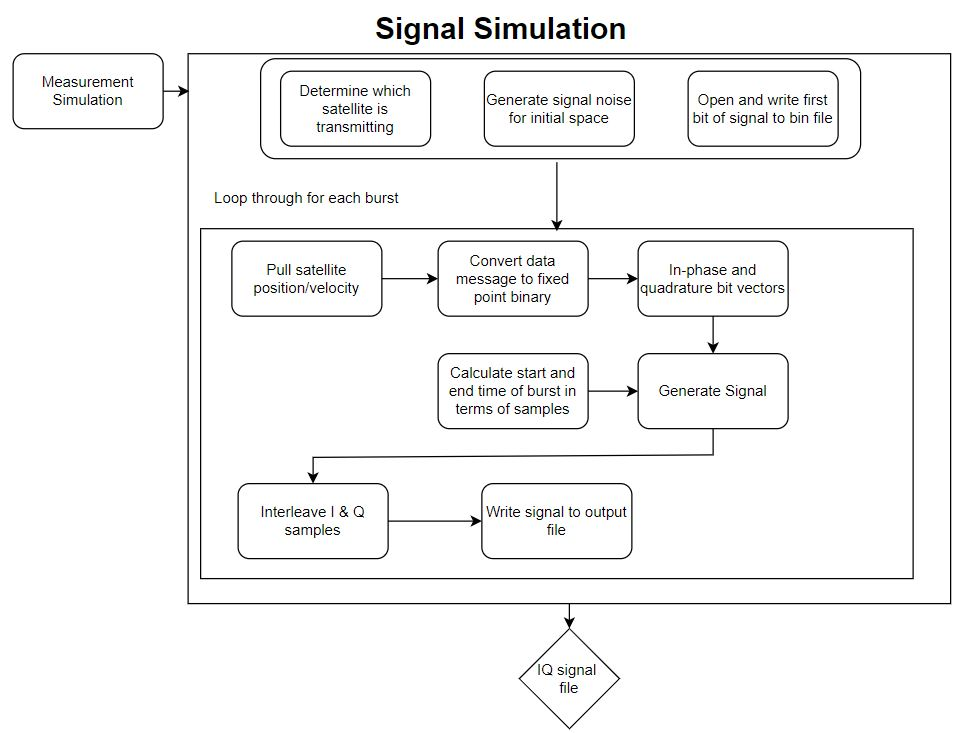
\includegraphics[width=4in]{SignalSimBlock}
    \caption{Signal Simulation Block Diagram}
    \label{fig:SigSimBlock}
\end{figure}

The main settings used for the signal simulation are as follows
\begin{itemize}
    \item Carrier frequency in Hz
    \item Carrier wavelength 
    \item Signal sampling frequency in Hz 
    \item Code frequency
    \item Symbols per burst
    \item Code period 
    \item Burst length in seconds
    \item Block size
    \item Signal noise power in decibels
    \item Signal noise power in watts
    \item Carrier to noise ratio
    \item Signal power in decibels
    \item Signal power in watts
    \item Noise toggle switch (on/off)
    \item Generate signal (on/off)
    \item Burst time in seconds
\end{itemize}
The following subsections will procede as follows: initial calculations, data message generation, and signal generation.

\subsection{Initial Calculations}
Initial calculations that are made for the signal simulation are initial signal noise and satellite transmission determination. Since the beginning of the simulation begins the transmission of a burst and the simulation is based on the what is seen by the receiver, an initial section of noise must be calculated to account for the transmission of the initial burst. Also, since only one burst occurs within the specified burst period, satellites must be chosen to transmit at specific times. The inputs for this section are as follows:
\begin{description}
    \item[Signal Noise Toggle] The signal noise toggle switch is used to turn on and off the signal noise. 
    \item[Signal Noise] The power of the noise floor.
    \item[Sampling Frequency] The sampling frequency of the signal in Hz.
\end{description}

The simulation starts by determining what satellite is transmitting and stores it into an array. This process is probabilistic and one satellite in view is chosen at random to transmit. This process is performed for each burst at the start of the signal simulation. Once the burst transmission list has been determined, the first part of the signal is generated. The first part of the output file will be signal noise. The signal noise will be the length of the first transit time in terms of samples. For example, if the first transit time is 0.003009 seconds and the sampling frequency is one megahertz, the first 3009 samples will be noise. Next a bin file is generated and signal noise is written to the file. 

\subsection{Data Message Generation}
The data message is a part of the signal used to gain information about the object transmitting the signal. For satellites, the data message is a package of numerical values representing the state of the satellite. This can be the satellite position and velocity, orbital elements, clock states, etc. With the calculated received times and designated satellites, the signal can be generated in blocks started by gathering the information for the data message. For this simulation, there are two options for a navigation message. The first option is to broadcast the satellite positions and velocities at the time of broadcast, or the Kepler orbit parameters at the time of transmission can be used. Next, those terms are converted into fixed point binary strings. The data bits are generated in a separate function that is specific to the data message type. The length of each word is predetermined inside the data bit generation function.  The fractional length is determine based on the amount of precision the user desires. The decision to sign the word is also declared. The branch of in-phase or quadrature has also been predetermined. The outputs of the bit generation function are two row vectors of in-phase and quadrature bits. Non return to zero (NRZ) coding is used to represent the binary ones and zeros. Next, the number of samples in the signal block is determined by examining the begin time of the current burst and the begin time of the next burst. The difference in time is calculated and multiplied it by the signal sampling frequency in order to calculate the number of samples in the block. Options for the data message types can be seen in table \ref{table:SVPosDataMes} and table \ref{table:COEdatMes} below.

\begin{table}
\begin{center}
\begin{tabular}{|c|c|c|c|}
    \hline
    Satellite Position and Velocity ECEF \\
    \hline\hline
    Term & Total bits & Fractional bits & Branch \\
    \hline
    Satellite ID & 8 & 0 & Q \\
    \hline
    Satellite Pos. & 32 & 7 & Q \\
    \hline
    Satellite Vel. & 32 & 7 & Q \\
    \hline
    Transmit Time & 64 & 0 & I \\
    \hline
\end{tabular}
\caption{Satellite Position and Velocity Data Message}
\label{table:SVPosDataMes}
\end{center}
\end{table}

\begin{table}
    \begin{center}
        \begin{tabular}{|c|c|c|c|}
            \hline
            Kepler Elements \\
            \hline\hline
            Term & Total bits & Fractional bits & Branch \\
            \hline
            Sat ID & 8 & 0 & I \\
            \hline
            \textit{h} & 48 & 32 & Q \\
            \hline
            \textit{e} & 48 & 57 & Q \\
            \hline
            \textit{RAAN} & 48 & 45 & Q \\
            \hline
            \textit{i} & 48 & 47 & Q \\
            \hline
            \textit{w} & 48 & 47 & Q \\
            \hline
            \textit{TA} & 48 & 45 & Q \\
            \hline
            \textit{a} & 48 & 35 & Q \\
            \hline
            Transmit time & 48 & 17 & I \\
            \hline
        \end{tabular}
    \end{center}
    \caption{COE Data Message}
    \label{table:COEdatMes}
\end{table}
The satellite positions and velocities mentioned in table \ref{table:SVPosDataMes} are for each individual cartesian component of the satellite position and velocity.

\subsection{Signal Generation}
Next is the generation of the signal shown in figure \ref{fig:SigGenBlock}. This is where all parts of the signal are combined together and generated. 

\begin{figure}[h]
    \centering
    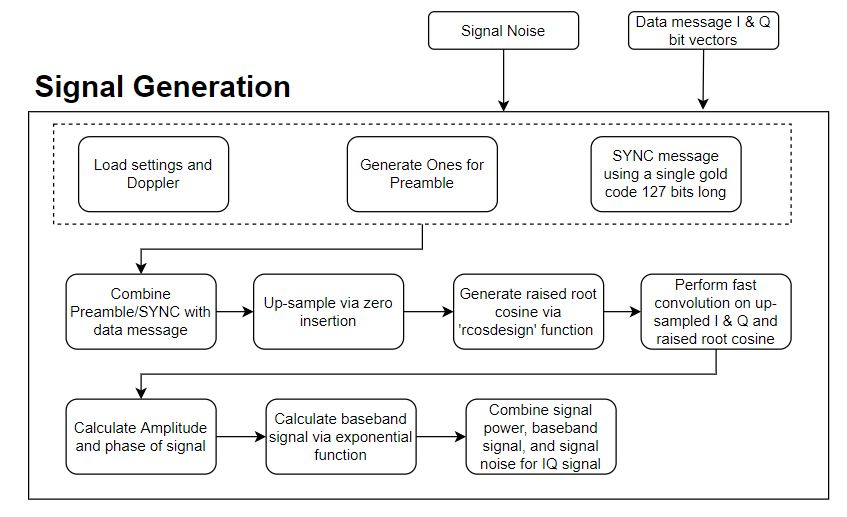
\includegraphics[width=3.5in]{SignalGenBlockDiagram}
    \caption{Signal Generation Block Diagram}
    \label{fig:SigGenBlock}
\end{figure}
The inputs to the signal generation block are as follows:
\begin{description}
    \item[Signal power] The power of the signal.
    \item[Sampling frequency] The sampling frequency of the signal in Hz.
    \item[Block size] The size of the block in terms of samples.
    \item[Doppler frequency] The previously calculated received Doppler frequency. 
    \item[Signal noise] A section of signal noise generated for the length of the burst.
    \item[Data message] The in-phase and quadrature bit vectors of the data message.
\end{description}

A section of signal noise is generated for the amount of samples in the signal block. The sync message and preamble are a set of alphanumeric values that when converted to binary values have good autocorrelation properties \cite{dinanSpreadingCodesDirect1998}. The autocorrelation is important for the receiving and decoding of the signal and will be discussed further in this chapter. The preamble and sync messages are combined to their respective branches along with the in-phase and quadrature bit vectors to produce the full data message. If the number of bits used by the data message is lower than the number of bits in the burst, the remaining bits will be assigned random binary values. Up-sampleing via zero insertion and filtering with a root-raised-cosine (RRC) pulse shaping filter is performed. The signal has to be up-sampled in order to meet the requirements set by the sampling frequency. The amplitude of the signal is calculated as equation \ref{eqn:amplitude} and the phase is calculated in equation \ref{eqn:phase}

\begin{equation}
    A = \sqrt{Ips^2 + Qps^2}
    \label{eqn:amplitude}
\end{equation}

\begin{equation}
    \theta = tan^{-1} \frac{Qps}{Ips}
    \label{eqn:phase}
\end{equation}
where \textit{Ips} and \textit{Qps} are the pulse shaped in-phase and quadrature branches respectively. The signal is generated through an exponential function in equation \ref{eqn:signal}

\begin{equation}
    A e^{j2\pi (f_{Doppler}t + \theta)}
    \label{eqn:signal}
\end{equation}
where \textit{A} is the amplitude and $\theta$ is the phase. From here the declared signal power is added along side the signal noise. The output of the signal generation function is a full IQ signal with signal noise. The signal is then split into real and imaginary parts, where they are interleaved and written to the bin file. To save computational memory, the signal variables are cleared with each iteration. This process is performed for each block of signal throughout the simulation. At the end of the simulation, if there is a received time outside the bounds of the simulation time, then the simulation will end the file with signal noise.

\subsection{Final Outputs}
The final outputs of the signal simulation are as follows:
\begin{description}
    \item[Bin file] A bin file with the generated signal where the real and imaginary parts of the signal have been interleaved.
    \item[I and Q bit matrix] A matrix with the in-phase and quadrature bit vectors of each burst are saved. These values are saved for analysis of bit rate error that will be observed in the results section of this thesis.
    \item[Navigation Data] A matrix of navigation data which includes the satellite number, satellite states, and transmit time for each burst is saved for analytical purposes later in this thesis.
\end{description}
\section{Receiver}
For this thesis, a specialized receiver was designed to process the data. 
- Include stuff about burst receiver

- Maximum likilehood burst detection
    - find source for this so I can talk about it in detail.

- Decoding of the bits

- Receiver outputs. Decoded Navigation Message, Doppler Frequency, location of the bit (to get a range), Failed bursts, Successful Bursts, output bits for bit error calculation,

\chapter{Testing Setup and Positioning Techniques}
This chapter will discuss positioning techniques used for validation of results in this thesis. Two specific positioning techniques are Doppler based and Pseudorange based. These techniques will be used along with the outputs of the receiver in order to gain a positioning solution.
 
\section{Doppler Based Positioning} \label{sec:DopplerPosTechnique}
Doppler positioning is not a new technique. In fact it was used with the original TRANSIT sytem in the 1960's and positioning accuracy was found to be within 500 meters. Doppler shift occurs as a result of a transmitter moving relative to an observer. As the transmitter moves closer, the frequency of the signal increases as the wave is being pushed closer to the observer. The opposite is true as the transmitter moves away from the user. The basis of Doppler positioning is using the change in signal frequency to gain an understanding of the motion of the transmitter. That information along with known satellite states can be used to gain a positioning solution.

The outputs of the receiver detailed in this thesis include the satellite position vector $\mathbf{r_{sv}}$, the satellite velocity vector $\mathbf{v_{sv}}$ and the received Doppler frequency $f_{Doppler}$. By rearanging \ref{eqn:doppler}, the pseudorange rate of the $k^{th}$ satellite can be calculated in \ref{eqn:prrfromdoppler}.

\begin{equation}
    \dot{\rho^{k}} = f_{Doppler}^{k} \cdot -\lambda
    \label{eqn:prrfromdoppler}
\end{equation}

Using \ref{eqn:prrfromdoppler} and \ref{eqn:rangerate} to rearange \ref{eqn:pseudorangerate}, the following equation is developed.

\begin{equation}
    \dot{\rho^{k}} = (\mathbf{v^{k}} - \mathbf{v_u}) \cdot \frac{(\mathbf{x^k} - \mathbf{x_u})}{\| \mathbf{x^k} - \mathbf{x_u}\|} + \dot{b} + \epsilon^{k}
    \label{eqn:extendedprreqn}
\end{equation}
For a static receiver $\mathbf{v_u}$ in equation \ref{eqn:extendedprreqn} will be zero resulting in equation \ref{eqn:staticextendedprreqn}.

\begin{equation}
    \dot{\rho^{k}} = \mathbf{v^{k}} \cdot \frac{(\mathbf{x^k} - \mathbf{x_u})}{\| \mathbf{x^k} - \mathbf{x_u}\|} + \dot{b} + \epsilon^{k}
    \label{eqn:staticextendedprreqn}
\end{equation}

With knowledge of the satellite states from the decoded navigation message, the unknowns are $\mathbf{x_u}$ and $\dot{b}$, where
\begin{equation}
\mathbf{x_u} = 
\begin{bmatrix}
        x_u\\
        y_u\\
        z_u 
\end{bmatrix}.
\end{equation}
With four unknowns, at least four measurements will be needed to solve for a positioning solution. An iterative process can be used to solve for the unknowns. 
First, an initial estimate of the states must be made. This will be represented by
\begin{equation}
    \mathbf{\hat{x}} = 
    \begin{bmatrix}
        \hat{x}_u\\
        \hat{y}_u\\
        \hat{z}_u\\
        \hat{\dot{b}}
    \end{bmatrix}
    \label{eqn:dopplerestimates}
\end{equation}
where the $\mathbf{x}$ is the vector of all unknown states, including the clock term.
Next is a vector of pseudorange rate measurements from \ref{eqn:prrfromdoppler} taking the form
\begin{equation}
\mathbf{\dot{\rho}} = \begin{bmatrix}
    \dot{\rho}_1 \\
    \dot{\rho}_2 \\
    \vdots\\
    \dot{\rho}_n
\end{bmatrix}
\end{equation}
where $n$ is the number of measurements being used. Next an estimate of the pseudorange rate is calculated for each satellite by combining \ref{eqn:dopplerestimates} and \ref{eqn:staticextendedprreqn} to form 

\begin{equation}
    \mathbf{\hat{\dot{\rho}}} = \begin{bmatrix} 
        \mathbf{v_1} \cdot \frac{(\mathbf{x_1} - \mathbf{\hat{x_u}})}{\| \mathbf{x_1} - \mathbf{\hat{x_u}}\|} + \hat{\dot{b}} \\ 
        \mathbf{v_2} \cdot \frac{(\mathbf{x_2} - \mathbf{\hat{x_u}})}{\| \mathbf{x_2} - \mathbf{\hat{x_u}}\|} + \hat{\dot{b}} \\ 
        \vdots \\
        \mathbf{v_n} \cdot \frac{(\mathbf{x_n} - \mathbf{\hat{x_u}})}{\| \mathbf{x_n} - \mathbf{\hat{x_u}}\|} + \hat{\dot{b}} 
    \end{bmatrix}
    \label{eqn:pseudorangerateEstimate}
\end{equation}

The measurement matrix $\mathbf{H(\mathbf{\hat{x}})}$ takes the form below where it is an $n \times 4$ matrix, where $n$ is the number of measurements being used.
\begin{equation}
\mathbf{H(\mathbf{\hat{x}})} = \begin{bmatrix}
    \frac{(\mathbf{x_1} - \mathbf{\hat{x_u}})}{\| \mathbf{x_1} - \mathbf{\hat{x_u}}\|} \times \left(\frac{(\mathbf{x_1} - \mathbf{\hat{x_u}})}{\| \mathbf{x_1} - \mathbf{\hat{x_u}}\|} \times \frac{\mathbf{v_1}}{\| \mathbf{x_1} - \mathbf{\hat{x_u}}\|}\right) && 1 \\
    \frac{(\mathbf{x_2} - \mathbf{\hat{x_u}})}{\| \mathbf{x_2} - \mathbf{\hat{x_u}}\|} \times \left(\frac{(\mathbf{x_2} - \mathbf{\hat{x_u}})}{\| \mathbf{x_2} - \mathbf{\hat{x_u}}\|} \times \frac{\mathbf{v_2}}{\| \mathbf{x_2} - \mathbf{\hat{x_u}}\|}\right) && 1 \\
    \vdots && \vdots\\
    \frac{(\mathbf{x_n} - \mathbf{\hat{x_u}})}{\| \mathbf{x_n} - \mathbf{\hat{x_u}}\|} \times \left(\frac{(\mathbf{x_n} - \mathbf{\hat{x_u}})}{\| \mathbf{x_n} - \mathbf{\hat{x_u}}\|} \times \frac{\mathbf{v_n}}{\| \mathbf{x_n} - \mathbf{\hat{x_u}}\|}\right) && 1 \\
\end{bmatrix}
\label{eqn:DopplerHMatrix}
\end{equation}
With this form, an estimate of the position and clock drift can be calculated using an iterative process. The first step of the process is to fill in equation \ref{eqn:DopplerHMatrix} with the initial guess position guess, satellite positions, satellite velocities. The next process is to calculate the pseudorange rates using \ref{eqn:pseudorangerateEstimate}. The next process is to create a delta pseudorange rate using equation \ref{eqn:deltarangerate}.

\begin{equation}
\delta \mathbf{\dot{\rho}} = \mathbf{\dot{\rho}} - \mathbf{\hat{\dot{\rho}}}
\label{eqn:deltarangerate}
\end{equation}
By using the delta pseudorange rate, the error of the original estimate is what is being calculated. This is calculated through least squares shown in equation \ref{eqn:LeastSquares}.

\begin{equation}
\mathbf{\tilde{x}} = \mathbf{(H^TH)^T H^T \delta \dot{\rho}}
    \label{eqn:LeastSquares}
\end{equation}
The new position estimate is calculated through \ref{eqn:NextEstimateIteration}.
\begin{equation}
    \mathbf{\hat{x}_{new}} = \mathbf{\hat{x}_{old}} + \mathbf{\tilde{x}}
\label{eqn:NextEstimateIteration}
\end{equation}
This process is continued iteratively until some threshold is met. Once the threshold is met, the process is concluded and the position and clock drift are output.

This process is typically employed using four or more measurements at the same time. For this thesis, a batched technique will be used. Since the nature of the signal used in this thesis is discontinuous, only one measurement is received at each time. One way to combat this is to use batched measurements. Batching measurements means taking measurements over a select period of time and treating them as if they all have come at one time. The advantage of batching measurements is that it allows the user to have enough measurements to gain an accurate position. Typically, when batching measurements, many measurements must be used in order to gain geometric diversity appart from each other. One disadvantage of batching measurements is that it can take longer periods of time to gather enough measurements in order to gain a position estimate. Long term, the act of batching measurements is similar to averaging them all over time. 

\section{Pseudorange Based Positioning} \label{sec:PseudorangePosTechnique}
Pseudorange based positioning is also not a new concept. Pseudoranges are used to solve the trilateration problem discussed in section \ref{sec:satellitenav}. Equation \ref{eqn:pseudorange} previously discussed is the pseudorange equation. It includes the true range, satellite and receiver clock errors, atmospheric errors, and unmodeled effects. Similar to the Doppler positioning in section \ref{sec:DopplerPosTechnique}, an iterative process is used to solve for a positioning solution. However instead of using the range rate, the pseudorange is used. There are a few modifications that need to be made to the equations used in this process, however the process of solving for the position as a whole is quite similar. 
\begin{itemize}
    \item     - Mention things about the configuration:
    \item     - satellite orbits
    \item     - signal type
    \item     - USRP playback and record
    \item     - why important
    \item     - how it works
    \item     - how USRPs work in brief

\end{itemize}


\chapter{Results}

This chapter will be used to show the results from simulations run in this thesis. The purpose of these results is to show that the simulation tool is capable of producing a signal that gives realistic results. 

\section{Static Clean Data}
The data set generated for this scenario is a static data set with zero clock error, zero thermal signal noise, and zero atmospheric errors. The purpose of this experiment was to examine what the cleanest possible data set would produce.  
\subsection{Doppler Positioning}
The first positioning strategy for this data set is using the received Doppler measurements in a batched fashion using the equations in section \ref{sec:DopplerPosTechnique}. 
\begin{figure}[h!]
    \centering
    \includegraphics[trim=1.2in 3.3in 1.75in 3.3in,clip,width=5in]{Iridium Doppler Positioning from Cleanest Set.pdf}
    \caption{Position Estimate from Batched Doppler Measurements}
    \label{fig:cleaniriddopgeo}
\end{figure}

\begin{figure}[h!]
    \centering
    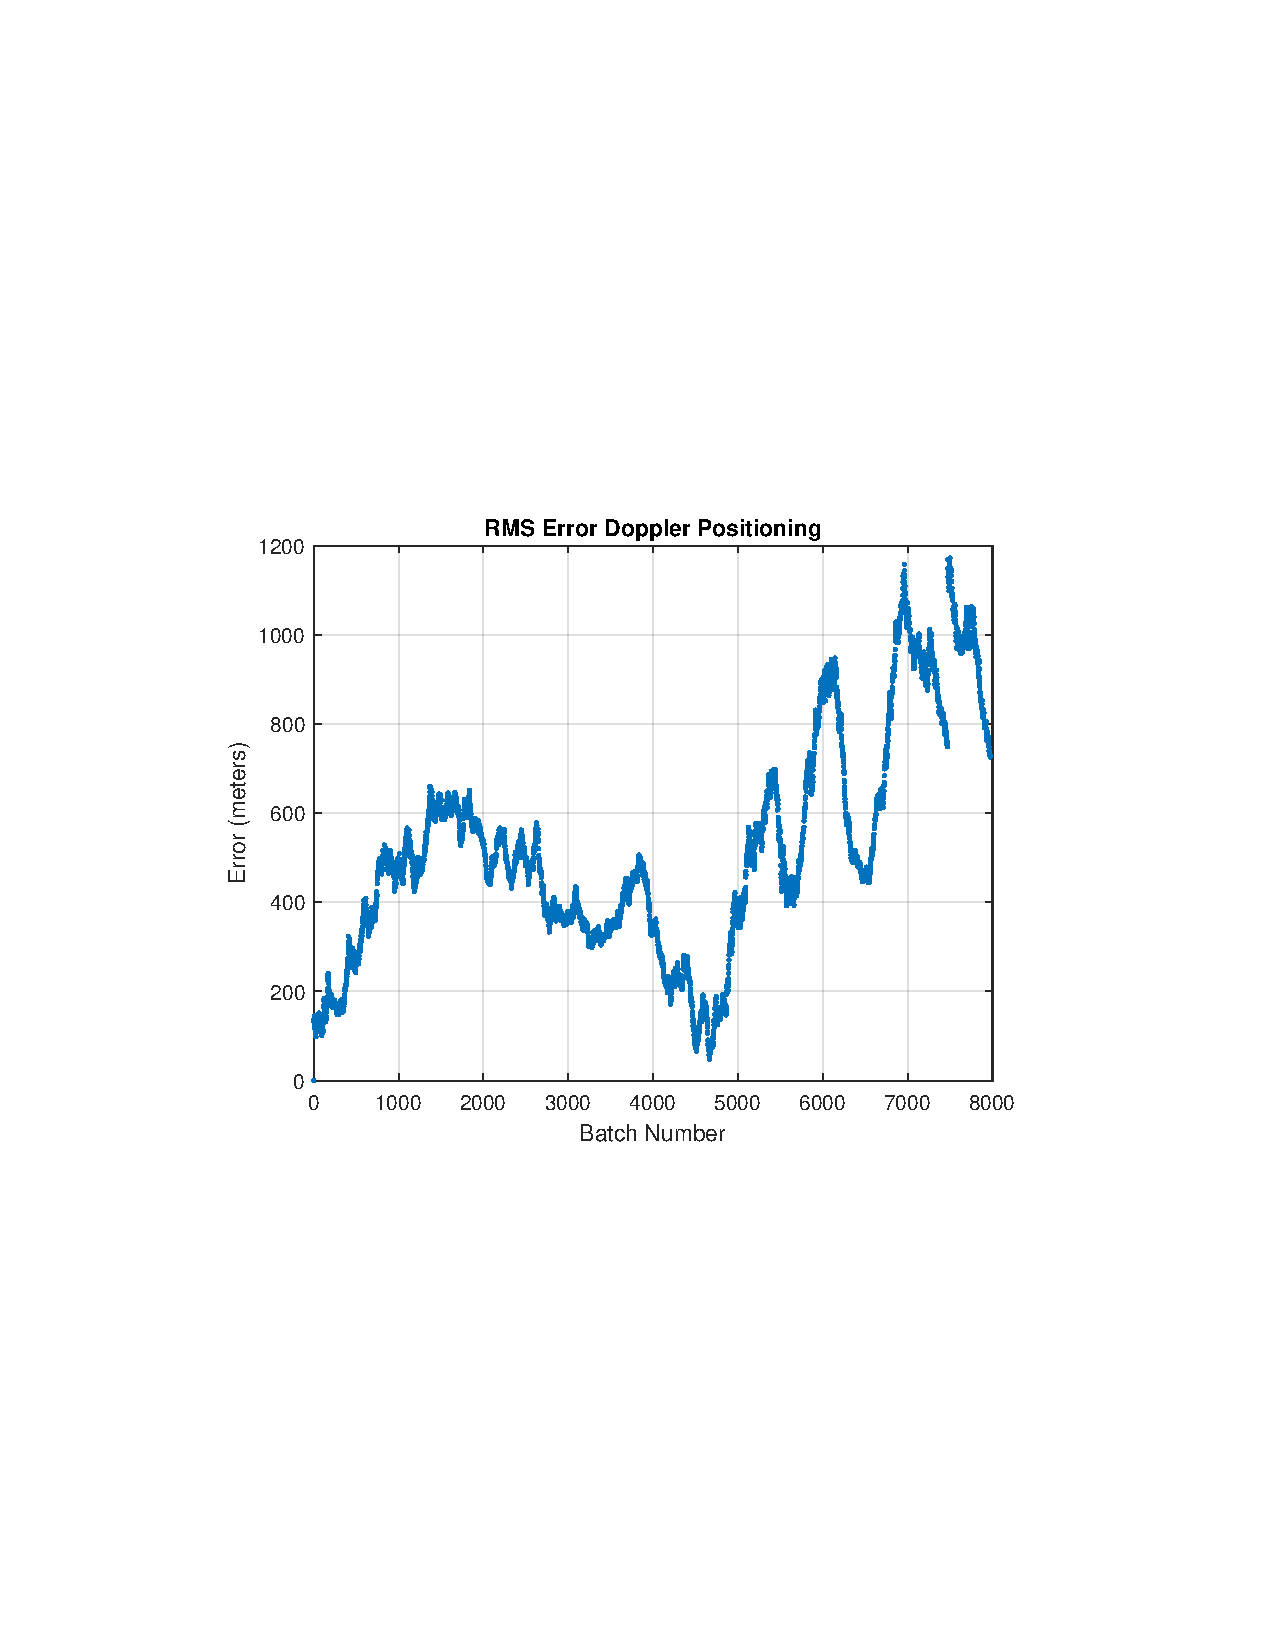
\includegraphics[trim=1.2in 3.3in 1.75in 3.3in,clip,width=5in]{Iridium RMSE plot Doppler Cleanest file.pdf}
    \caption{RMS Error of Batched Doppler Estimates}
    \label{fig:RMSErrorBatchDoppler}
\end{figure}


\subsection{Pseudorange Based Positioning}
\section{Static Clean Data Played Through USRP}
\subsection{Doppler Positioning}
\subsection{Pseudorange Based Positioning}
\section{Static Dirty Data}
\subsection{Doppler Positioning}
\subsection{Pseudorange Based Positioning}
\section{Dynamic Clean Data}
\section{Dynamic Clean Data Played Through USRP}
\section{Dynamic Dirty Data}
    - positioning results

    - Doppler Positioning 

    - comparison of constellations 

    - positioning algorithms

    - batch recursive least squares

    - 2d positioning and 3d positioning

    - possible aided doppler positioning techniques

    - How many bursts were detected and accurately decoded

    - Possible testing configurations   
        
        - Full clean data (no clock, no noise, no trop)

        - Full clean data run through USRP 

        - Simulated dirty set with trop error, clock error, sig noise

        - Run this simulation for 2 different satellite constellations

        - See if I have to run it for a dynamic rover 
            - Update:I do.




\chapter{Conclusions and Future Work}
- The simulator works well 

- addition of more signals

- addition of multiple constellation

- addition of more error terms





\bibliographystyle{unsrt}
\bibliography{MyLibrary}






\begin{appendix}
\chapter*{Appendices\addcontentsline{toc}{chapter}{Appendices}}


\begin{singlespace}


\end{singlespace}
\end{appendix}
\end{document}

